%%%%%%%%%%%%%%%%%%%%%%%%%%%%%%%%%%%%%%%%%%%%%%%%%%%%%%%%%%%%%%%
%
% Welcome to Overleaf --- just edit your LaTeX on the left,
% and we'll compile it for you on the right. If you open the
% 'Share' menu, you can invite other users to edit at the same
% time. See www.overleaf.com/learn for more info. Enjoy!
%
%%%%%%%%%%%%%%%%%%%%%%%%%%%%%%%%%%%%%%%%%%%%%%%%%%%%%%%%%%%%%%%

\documentclass{beamer}
\usetheme{Copenhagen}
\setbeamertemplate{navigation symbols}{}
\usepackage[utf8]{inputenc}
\usepackage{listings}
\usepackage{graphicx}
\usepackage[export]{adjustbox}
\graphicspath{ {./photos/} }

\title{Linux Empowered Automation for Developers}
\author{Gabriel Hanu}
\institute{UBB - Mathematics and Computer Science}
\date{2024}

\titlegraphic{
\includegraphics[width=0.3\linewidth]{gdsc}}

\begin{document}

\frame{\titlepage}

% 1 SLIDE
\begin{frame}

\frametitle{Why do I like Linux? }

    \begin{figure}

        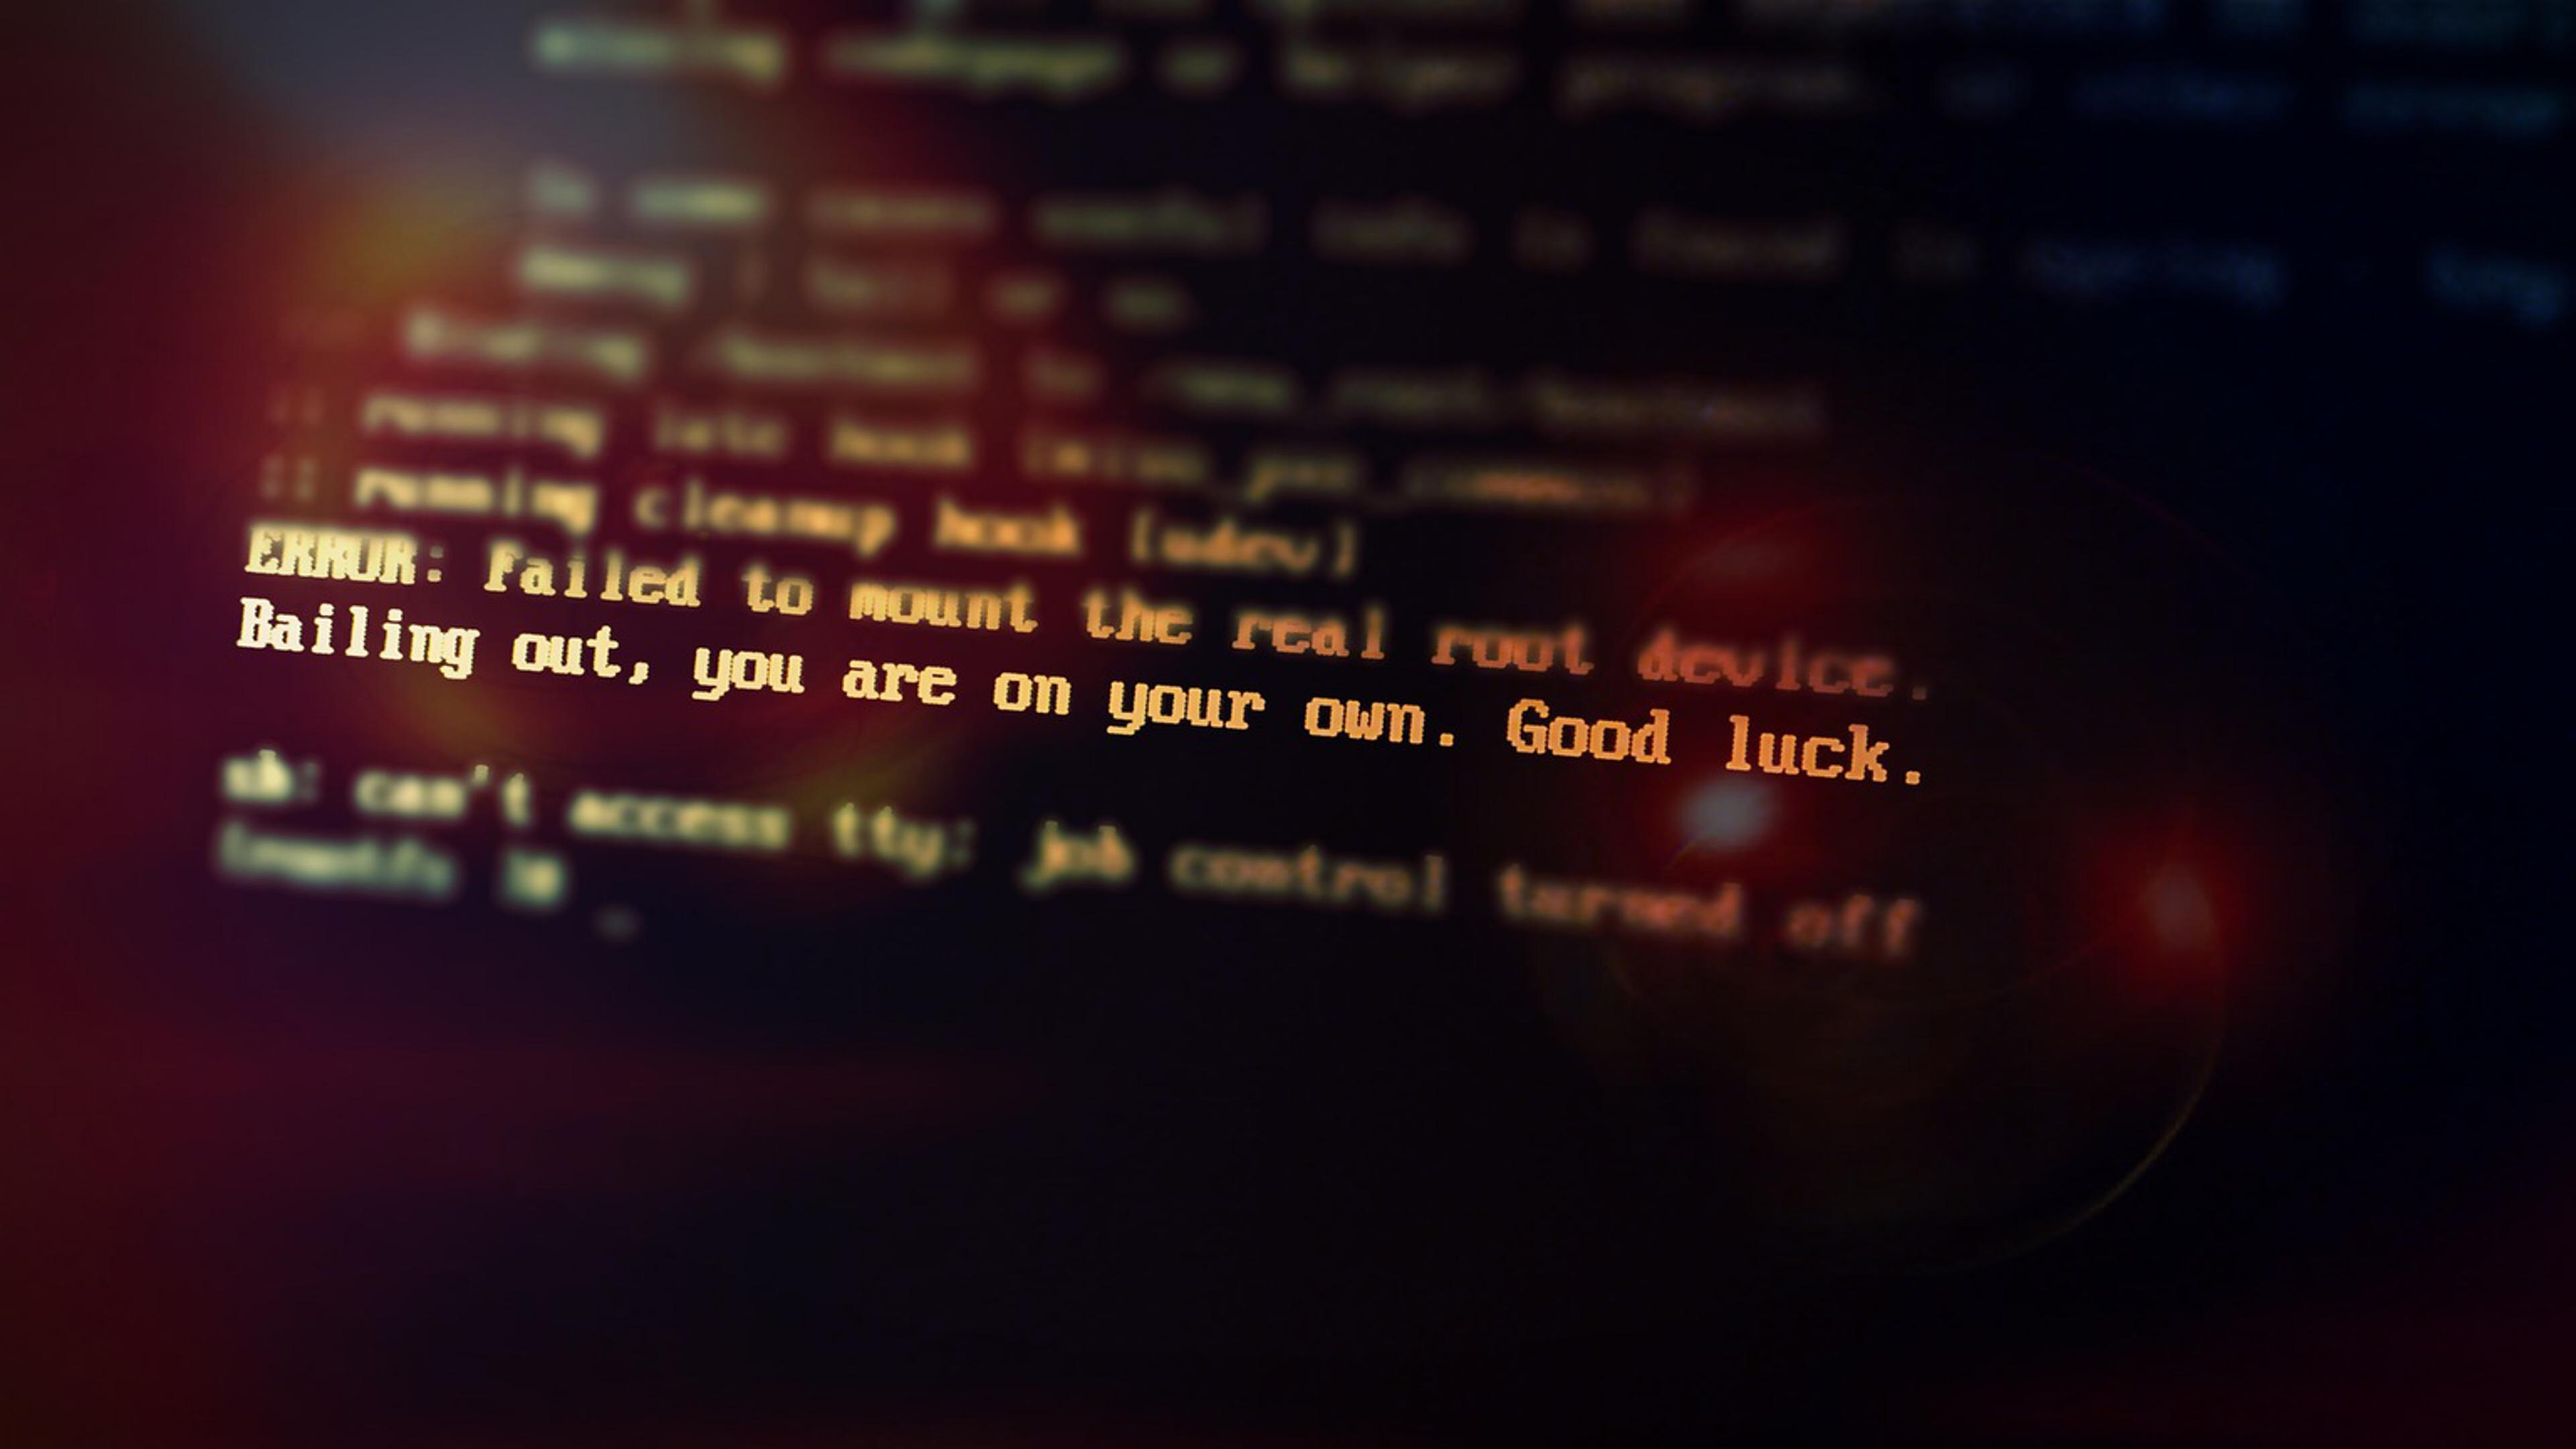
\includegraphics[width=0.8\linewidth]{whyilikelinux}

        \label{fig:whyilikelinux}

    \end{figure}
    \centering \small This may require a bit of a story...
\end{frame}

% 2 SLIDE
\begin{frame}

\frametitle{Useful resources}
\begin{itemize}
    \item Linux Bible
    \item Manual pages
    \item The wiki based on your distro (ex: ArchWiki)
    \item Reddit (r/linux), (r/linux4noobs), (r/linuxquestions)
    \item Youtube (Luke Smith, DistroTube, BugsWriter etc)
\end{itemize}

\small

.
\newline
also all the resources as well as the scripts and the thoroughly explained examples
will be available on my GitHub page.

\end{frame}

% 3 SLIDE
\begin{frame}
\frametitle{Quick notes}
\small I will introduce some basic concepts then dive into some examples and
will build up from there.
    \newline \newline
I want you to actively participate in the learning process. So you may try to guess
the output of some commands before I run them.
    \newline \newline
I may mess up during this process, so feel free to correct me.

\end{frame}

% 4 SLIDE
\begin{frame}
\frametitle{What will we cover today?}
\begin{itemize}
    \small
    \item Shell scripting (POSIX shell) \pause
    \item Cron jobs\pause
    \item Event-driven automation\pause
    \item Tmu\pause
    \item Kernel Modules
\end{itemize}

\end{frame}

% 5 SLIDE
\begin{frame}
\frametitle{Why is Linux so good at automation?}
\small
    Everything is a file (UNIX philosophy) \newline
    Open-source \newline
    Full control over the system \newline
    A lot of tools available \newline
    Very stable \newline

    The kernel and the init system exposes a lot of events that we can use to
    automate tasks.

\end{frame}

% 6 SLIDE
\begin{frame}
\frametitle{Setup the environment}
\small
    I use Arch based distribution, the difference is not that big, I don't use
    systemd but openrc. \newline
    But you can use any distro you want as long as you understand the differences

\end{frame}

% 8 SLIDE

\begin{frame}
\frametitle{How can a developer benefit?}
\small
the short answer is through automation. \newline
firstly one need to identify the repetitive tasks that can be automated.\newline
certain tasks have been singled out as being easily controllable.
    \begin{itemize}
        \item clean up old files
        \item backups
        \item hot reloading
        \item managing logs
        \item compiling and running projects
    \end{itemize}
    also you can propose your own tasks that you think can be automated and
    we can try to implement them.

\end{frame}


% 9 SLIDE
\begin{frame}
    \frametitle {Where do we start?}
    \small
    We should start by understanding the environment we are working in and how
    the tools interact with each other. \newline \newline
    For that I will have to draw a picture...
\end{frame}

\begin{frame}
    \frametitle{Environment}
    \small Usually on our machine we only have one user, but you have to
    take into consideartion the root as well. Also you can have multiple users
    asignated to different groups and tasks ( gaming )
    \newline
    \newline
    To see the environment variables you can use the command\newline
    \textbf{printenv} \newline
    then switch to another user and check again.\newline
    \textbf{su - root} \newline
    \textbf{printenv} \newline

    On most system there are a lot of variables and you can observe that
    some variables exists for a user and does not for another. \newline
    \newline
    Let's draw a bit to understand them...
\end{frame}


% 10 SLIDE
\begin{frame}
\frametitle{POSIX shell}
\small
I will not cover the basics of shell scripting, as there is a lot of resources available online and at the university.
    \newline \newline
Shell scripting may not read like a programming language, so everytime you
don't understand something, you can raise your hand and ask me to explain it!
    \begin{figure}
        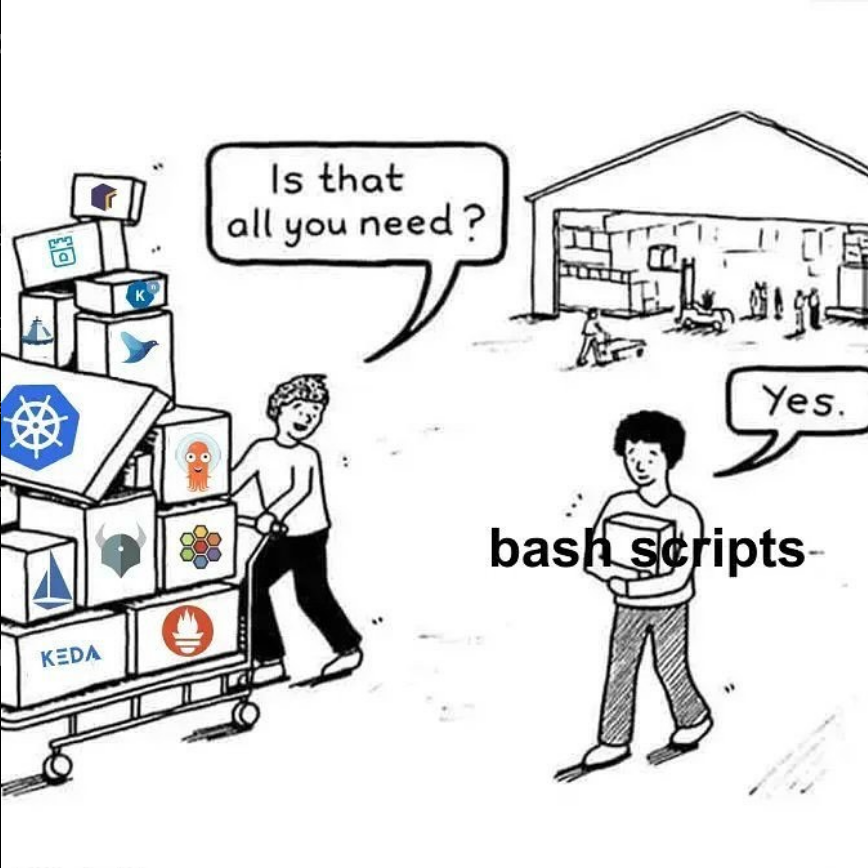
\includegraphics[width=0.4\linewidth] {bashgod}
        \label{fig:bashgod}
    \end{figure}

\end{frame}

\begin{frame}
    \frametitle{Where to place the scripts?}
    \small
    For the scripts that we will write today, we will place them in the directory
    of the github repostitory that I have created for this workshop.
    \newline \newline
    \textbf{But} in general you can place them in the following directories:
    \begin{itemize}
        \item /usr/local/bin
        \item /usr/bin
        \item /bin
        \item ~/.local/bin
    \end{itemize}
\end{frame}

% 11 SLIDE
\begin{frame}
    \frametitle{Our first automatization}
    \small We will start with a simple script that will clean up the trash
    \newline then we will backup configs and move on to create hot reloading
    on a generic project.
\end{frame}

% \begin{frame}
%     \frametitle{Let's talk debugging}
%     \footnotesize
%     The Bash shell contains no debugger, nor even any debugging-specific commands or constructs
%     \begin{figure}
%
%         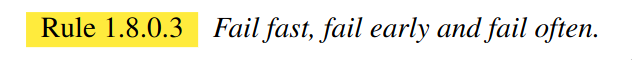
\includegraphics[width=0.6\linewidth, left]{fail}
%
%         \label{fig:fail}
%
%     \end{figure}
%     We have some tools to help us with that in shell scripting:
%     \begin{itemize}
%         \item set -x / -e / -u / -o pipefail
%         \item out beloved printf
%         \item dtrace
%         \item strace
%     \end{itemize}
% \end{frame}
%
\begin{frame}
    \frametitle{It's not that convienient to run manually a script}
    \small
    Now that we wrote a script that archives the old projects,
    maybe we will forget to run it at specific times or even worse, doing a while
    loop to check if the time has come.
\end{frame}

\begin{frame}
\frametitle{Now cron jobs comes into play}
\small
    One of the most useful tools for automation is cron. \newline
    It allows you to schedule tasks to run at specific times or intervals. \newline
    But there is more! \newline
\end{frame}

\begin{frame}
    \frametitle{How does cron/anacron work?}
    \small
    Cron is started from /etc/rc.d/init.d or /etc/init.d when classical sysvinit scripts are used. In case systemd is enabled, then unit file is installed into /lib/sys‐
       temd/system/crond.service and daemon is started by systemctl start crond.service command. It returns immediately, thus, there is no need to need to start it with  the
       \& parameter.
\end{frame}

\begin{frame}
    \frametitle{Anacron is a cron for laptops}
    \small
    Well, not only for laptops, but for systems that are not running 24/7. \newline
    Maybe you have a cron once 8 months, but you shut down your computer
    every day, then it is a high chanche to miss the job execution. \newline \newline
    It is a cron job that runs at boot time and checks if the cron jobs have been
    missed. \newline

\end{frame}

% 10 SLIDE
\begin{frame}
\frametitle{But there is more! Event driven automation}
\small
    What if we could automate tasks based on events that happen on the system? \newline
    \pause
    In this context, we can take advantage of the Linux kernel's ability to
    notify userspace programs of events that happen on the system. \newline
\end{frame}

% 11 SLIDE
\begin{frame}
\frametitle{What are the events in Linux that we can use?}
    \small
    \begin{block}{Remark}
        We will modify the behavior of the system based on the events throughout
        custom scripts, whose path may differ from one distro to another.
    \end{block}
    \begin{itemize}
        \item openrc/systemd daemons events (init system)
        \item inotify (file system events)
        \item cgroups (resource management)
        \item acpi (power driven events)
        \item udev (device management)
        \item custom hooks and signals
    \end{itemize}
\end{frame}

% 12 SLIDE
\begin{frame}
    \frametitle{Do you really need to compose all the events?}
    \small
    Absolutely not! \newline
    You can use the events that are relevant to your day to day tasks. \newline
\end{frame}

\begin{frame}
    \frametitle{Inotify - the file system events}
    \small
    Inotify is a Linux kernel subsystem that acts to extend filesystems to
    notice changes to the filesystem, and report those changes to
    applications. \newline
    \newline
    It can be used to modify the create, delete, modify, move etc events
    that happen on the filesystem. \newline
    \newline
    Let's look into an example with hot reloading a C++ program.
\end{frame}

\begin{frame}
    \frametitle{Other neat tricks}
    \small
    How about never crash your system out of the blue? \newline
    \newline
    You can use cgroups to limit the resources that a process can use. \newline
\end{frame}

\begin{frame}
    \frametitle{Orchestrating multiple projects with Tmux}
    \small
    Of course we will use Tmux to manage multiple projects.\newline
    \begin{figure}
        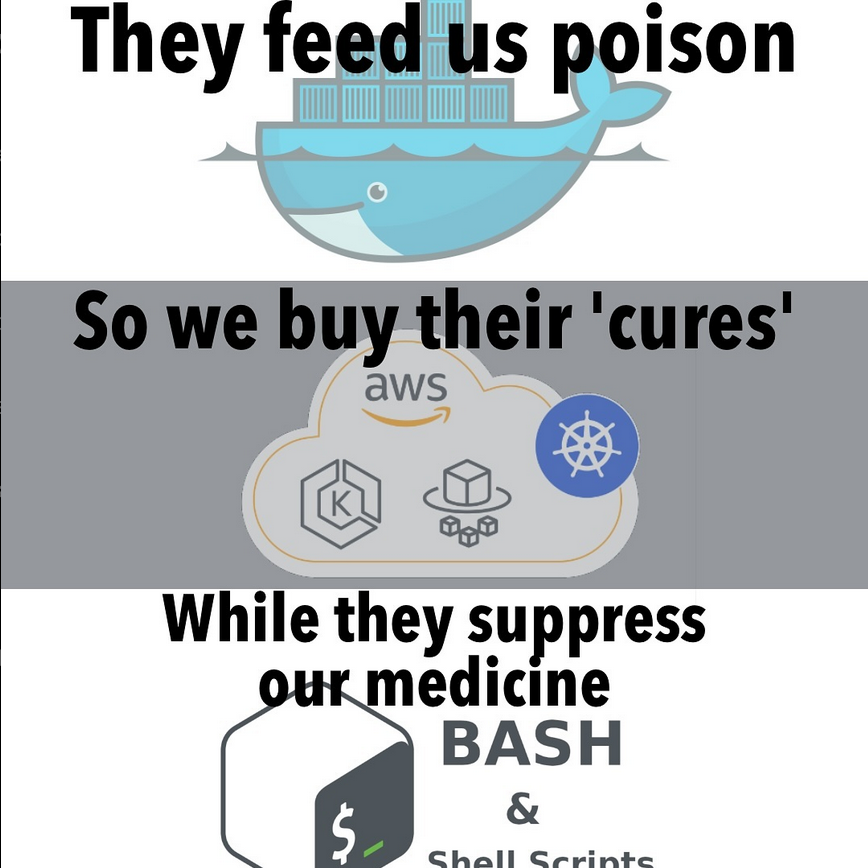
\includegraphics[width=0.4\linewidth] {bash_poison}
        \label{fig:bash_poison}
    \end{figure}
    \footnotesize \centering \textbf{Don't forget to poison the docker}
    it's convienient to use Docker for this task.
\end{frame}

\begin{frame}
    \frametitle{Getting your feed wet with Tmux}
    What is this Tmux thing?
    \newline
    \newline
    It's very simple to use but it can be scaled to a more complex situation
    at your work or to your personal projects.
    \newline \newline
    Let's see how we can use it to manage multiple projects.
\end{frame}
% 18 SLIDE
\begin{frame}
    \frametitle{Take it to the final level with Kernel Modules}
    \begin{figure}
        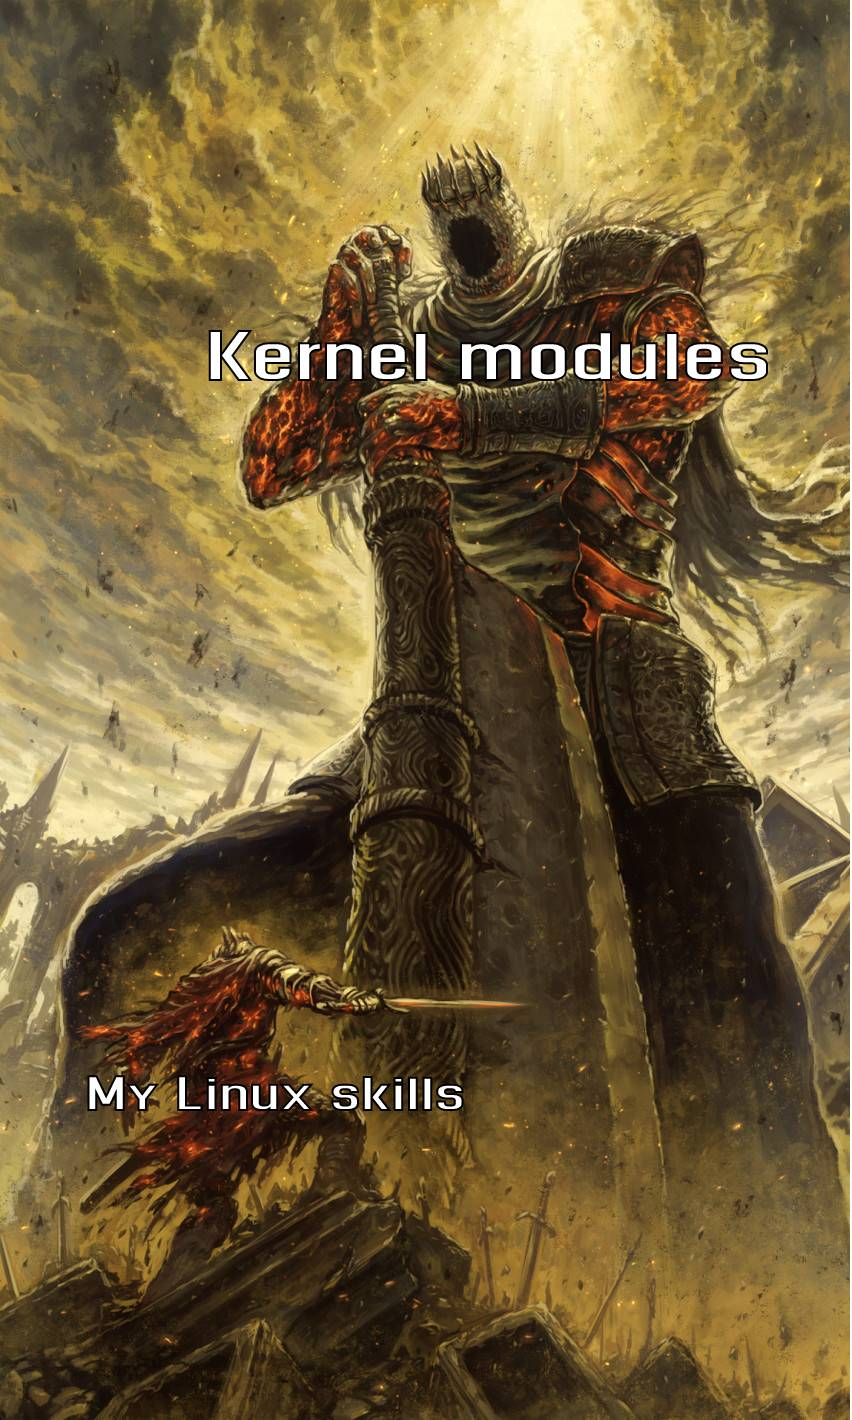
\includegraphics[width=0.35\linewidth] {linuxkernel}
        \label{fig:linuxkernel}
    \end{figure}
    \centering \small{Why do we need kernel modules anyway?}
\end{frame}

\begin{frame}
    \frametitle{Writing your own kernel module}
    \begin{alertblock}{Be aware of the risks}
        \small
        Writing a kernel module is a risky business, as it can crash the system
        if not done properly. \newline
        \newline
        \textbf{But} it can also be a very rewarding experience, as you will
        learn a lot about the kernel and the way it interacts with the hardware.
    \end{alertblock}
    \small
    The risks consists in the fact that you can write to the wrong memory
    address, you can cause a kernel panic, you can cause a deadlock, you can
    cause a memory leak, you can cause a buffer overflow etc.
    \newline
    Also you need to \textbf{pay attention to the future kernel releaseas} as
    the API may change and so your module should do.

\end{frame}

\begin{frame}
    \frametitle{Here we don't have int main() function...}
    \small
    Get rid of the main function, printf, scanf and other functions that are
    not available in the kernel space. \newline \newline
    A kernel module is a piece of code that can be loaded or unloaded
    from the kernel on demand. Hence there will be 2 functions that will
    handle this process: \newline
\end{frame}

\begin{frame}
    \frametitle{Load, unload, debug, repeat}
    \footnotesize
    A basic kernel module consists of the main file and the Makefile.
    \begin{figure}
        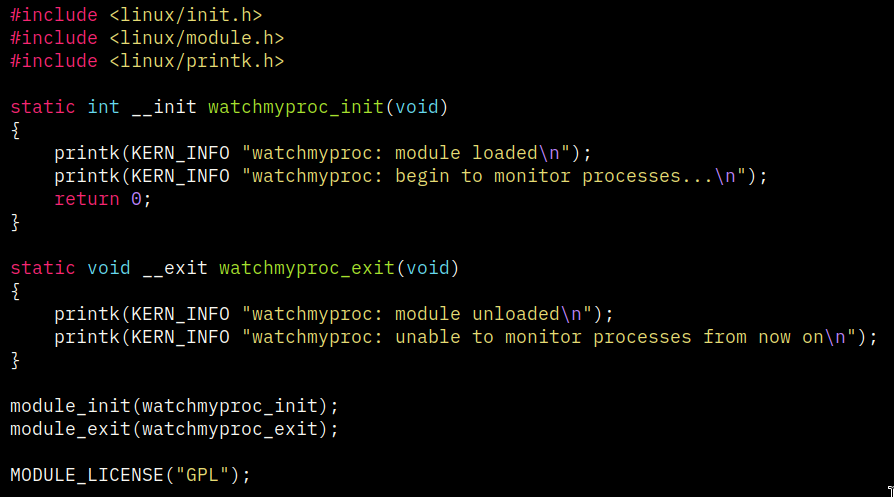
\includegraphics[width=0.7\linewidth] {simplekernel}
        \label{fig:simplekernel}
    \end{figure}
    Now you can compile it with:
    \textbf{make}
    \newline
    and load it with:
    \textbf{sudo insmod watchmyproc.ko}
    \newline
    check the output with:
    \textbf{sudo dmesg}
    \newline
    now you can remove it with:
    \textbf{sudo rmmod watchmyproc}
    \newline
    check the output again to see the module being removed.

\end{frame}

\begin{frame}
    \frametitle{Let the fun begin}
    \small
    We will utilize the kernel module to analyze the network trafiic that is
    running on the system and log the source and destination of the packets
    we will receive.
    \newline
    \newline
    We will take advantage of the kernel's ability to notify userspace
    throughout its API.
    \newline
    \newline
    Until now we have used programs that have exposed the kernel API to us
    \textbf{but} now we will use them directly with all the functions
    that are available to us.
\end{frame}

\begin{frame}
    \frametitle{Let's analyze the kernel module}
    \small oh boy isn't that fun?
\end{frame}

\begin{frame}
    \frametitle{Resources}
    \small
    I have documented everything in a github repository, where you can find it here:
    \begin{figure}

        
\includegraphics[width=0.4\linewidth]{qr-github}

        \label{fig:qr-github}

    \end{figure}
    \centering \small There will be links, examples we've done today and some
    extra resources for the adventurous ones that want to take the Linux
    journey to the next level.

\end{frame}

\begin{frame}
    \frametitle{Your feedback is important}
    \small
    This is my first workshop and I would like to know your opinion about it.
    \begin{figure}

        
\includegraphics[width=0.4\linewidth]{qr-github}

        \label{fig:qr-github}

    \end{figure}
    \centering \small Please scan the QR code and fill in the form.
\end{frame}

\begin{frame}
    \frametitle{Thank you!}
    \small
    I hope you enjoyed this workshop and that you have learned something new.
    \newline
    \newline
    Now we will have some time to answer your questions.
    \newline
    \newline
    So feel free to ask me anything you want to know.
\end{frame}

\end{document}
